\begin{figure}[h]
    \centering
    \setlength{\tikzunit}{.085\textwidth}
    \begin{tikzpicture}[scale=1.0,x=\tikzunit,y=\tikzunit]
% ---- Draw a grid which should help to position things -----------
%        \draw[step= .5,color=gray,thin,dashed] (-4,-4) grid (4,4);
%        \draw[step=1.0,color=gray]             (-4,-4) grid (4,4);
%        \draw[step=4.0,color=black]            (-4,-4) grid (4,4);
%  Notes:
%       just uncomment the lines with draw commands and the grid
%       will appear.  The commands, I believe are self explanatory
%       and it can be drawn as big as you want. The two coordinates
%       denote lower left and upper right corners of the grid.
% -----------------------------------------------------------------
        \node(0,0){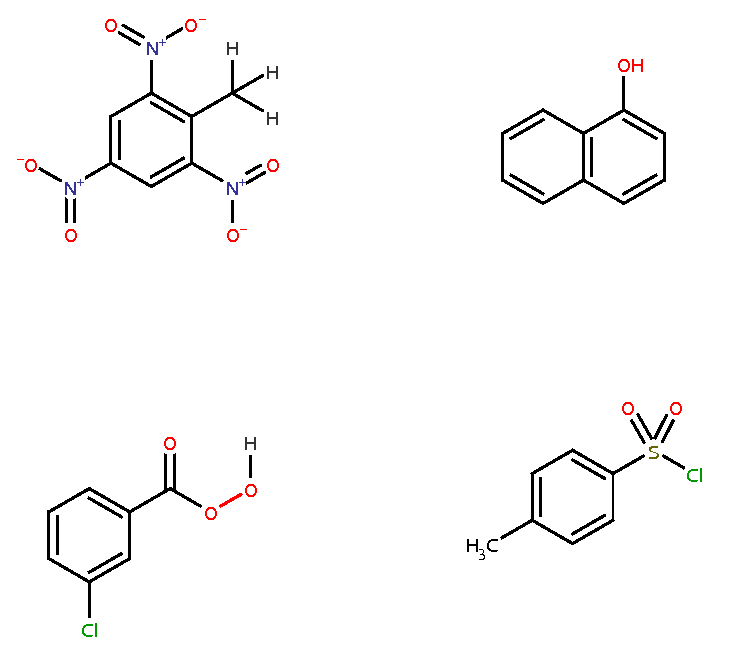
\includegraphics[width=7\tikzunit]{4struct.eps}};
        \draw (-2.1, 0.5) node{TNT};
        \draw ( 2.1, 0.5) node{Naphtol};
        \draw (-2.1,-3.5) node{\compx{1}};
        \draw ( 2.1,-3.5) node{\compx{2}};
    \end{tikzpicture}
    \caption{Overlaying \LaTeX\ commands to get some nice things.}
    \label{fig:struct1-2}
\end{figure}
